% Generated artifacts (paths relative to paper/): figures/TABLE_agents.tex, figures/TABLE_soundness.tex,
% figures/fig_coverage.pdf. Regenerate with figures/gen_*.py (see figures/README_FIGURES.md). Captions state the
% comparison first; every number below is printed by the generator scripts.

% === Table 1: agent stability and accuracy (E4 v5) ===
\begin{table*}[t]
  \caption{The hybrid and strict policies remove nearly all preview-induced changes in agent behavior; their accuracy
  differences to raw are indistinguishable from zero except for the strict policy on phi-4 ($-3.6$ points). Tasks (of
  150 BIRD tasks) whose
  trajectory (Traj.) or answer correctness (Corr.) changed across the three physical orders of the same database
  (1 thread) or between 1 and 8 threads on the original order (smart-lex was not run at 8 threads), per tool policy,
  in the final agent run; accuracy (Acc., \%) is BIRD execution accuracy averaged over
  the three orders; $\Delta$Acc is the paired difference to raw (percentage points, task-clustered bootstrap 95\% CI).
  Greedy decoding; identical prompts share one generation, so every change is caused by a differing observation.}
  \label{tab:agents}
  \centering\small
  \begin{tabular}{@{}ll rrrr rrrr@{}}
\toprule
 & & \multicolumn{4}{c}{Qwen3-8B} & \multicolumn{4}{c}{phi-4} \\
\cmidrule(lr){3-6}\cmidrule(l){7-10}
Executions & Policy & Traj. & Corr. & Acc. & $\Delta$Acc [95\% CI] & Traj. & Corr. & Acc. & $\Delta$Acc [95\% CI] \\
\midrule
Physical order & Raw & 61 & 16 & 52.4 & -- & 31 & 4 & 44.4 & -- \\
 & Smart-lex & 5 & 0 & 53.3 & $+0.9$ [$-2.9$, $+4.9$] & 1 & 0 & 44.0 & $-0.4$ [$-2.2$, $+1.1$] \\
 & Hybrid & 6 & 1 & 51.5 & $-0.9$ [$-4.2$, $+2.2$] & 1 & 0 & 45.3 & $+0.9$ [$-0.2$, $+2.4$] \\
 & Strict & 2 & 0 & 54.7 & $+2.2$ [$-1.8$, $+6.2$] & 0 & 0 & 41.3 & $-3.1$ [$-6.9$, $0.0$] \\
\bottomrule
\end{tabular}

\end{table*}

% === Table 2: soundness across probe sets and engines ===
\begin{table*}[t]
  \caption{Among complete supported statements, no preview produced by a certified DET/NARROW/ALL execution
  diverged; smart-lex was also stable on those same statements. Statements whose rendered preview (header, first 20
  rows, exact count) differed across equivalent executions: DuckDB with original and two permuted physical orders at 1 and 8 threads
  plus a repeated run (7 configurations); PostgreSQL with original and permuted heap order, serial and
  parallel-enabled, plus a repeated run (5 configurations). Supported = certificate DET/NARROW/ALL in the engine's
  dialect; censored statements lacked an observation in some configuration (or, on PostgreSQL, could not be
  translated). On UNSUPPORTED statements smart-lex offers no guarantee, and some still diverge.}
  \label{tab:soundness}
  \centering\small
  \begin{tabular}{@{}ll rrrr rrr@{}}
\toprule
 & & \multicolumn{4}{c}{Supported (DET/NARROW/ALL)} & \multicolumn{3}{c}{UNSUPPORTED} \\
\cmidrule(lr){3-6}\cmidrule(l){7-9}
Statements & Engine & $n$ (+cens.) & Certified rewrite & Smart-lex & Raw & $n$ (+cens.) & Raw & Smart-lex \\
\midrule
Development (1,015) & DuckDB & 854 (+0) & 0 & 0 & 378 & 161 (+0) & 69 & 39 \\
 & PostgreSQL & 836 (+17) & 0 & 0 & 285 & 157 (+5) & 51 & 32 \\
\midrule
Held-out (1,125) & DuckDB & 776 (+0) & 0 & 0 & 292 & 349 (+0) & 134 & 66 \\
 & PostgreSQL & 759 (+10) & 0 & 0 & 237 & 346 (+10) & 77 & 42 \\
\midrule
Unseen tasks I (1,321) & DuckDB & 999 (+0) & 0 & 0 & 394 & 322 (+0) & 92 & 44 \\
 & PostgreSQL & 978 (+16) & 0 & 0 & 301 & 295 (+32) & 61 & 32 \\
\midrule
Unseen tasks II (1,267) & DuckDB & 945 (+0) & 0 & 0 & 344 & 322 (+0) & 79 & 31 \\
 & PostgreSQL & 930 (+9) & 0 & 0 & 276 & 302 (+26) & 58 & 24 \\
\bottomrule
\end{tabular}

\end{table*}

% === Figure 3: coverage and narrowness ===
\begin{figure}[t]
  \centering
  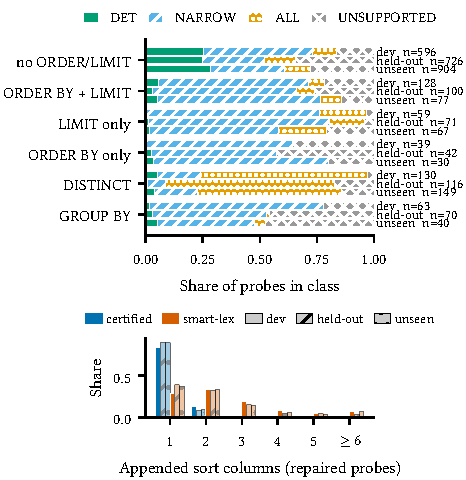
\includegraphics[width=\columnwidth]{figures/fig_coverage.pdf}
  \caption{Most previews are already determined or need one extra sort column. Top: certificate verdicts by probe
  class for the 1,015 development probes and the 1,125 held-out statements ($n$ per bar at right); ALL means the
  certified tie-break is no narrower than smart-lex's, not necessarily all output columns. Bottom: sort columns
  appended to the repaired (NARROW or ALL) probes ($n=689$ and $588$); the certified tie-break needs one column for
  84\% (development) and 90\% (held-out) of them, smart-lex for 29\% and 39\%.}
  \label{fig:coverage}
\end{figure}

% === Figure 1 (hero) and Figure 2 (certifier pipeline): figure-spec, see figures/specs/ ===
% === Table 3: observation cost (final E3) ===
\begin{table*}[t]
  \caption{Certification does not change the typical cost of an observation, and the predeclared cost bar is not met
  on either engine. Total time of one observation (preview under the policy + the exact count, identical for all
  policies) over one fixed probe set per engine at its largest replicated scale (a stress test, not a representative
  workload); median of five repetitions per probe. Change is certified vs smart-lex with a probe-bootstrap 95\% CI;
  median ratio is the per-probe smart-lex/certified ratio; top-5 left out is the change after removing the five probes
  that contribute most to the difference; the LIMIT class is LIMIT without a total order, where the bar asks for
  $\geq 5\times$ (and $\geq 20\%$ lower total overall). On PostgreSQL, two probes for which the key tie-break led the
  planner to an index-ordered nested loop account for most of the higher total. The main set excludes probes that fail
  at scale (18 per engine) and probes with a 60\,s timeout under any policy (2 on DuckDB, 8 on PostgreSQL); counting
  those timeouts at 60\,s as lower bounds gives $-0.7\%$ (DuckDB) and $+35.2\%$ [$-9.3\%$, $+123.7\%$] (PostgreSQL).}
  \label{tab:cost}
  \centering\small
  \begin{tabular}{@{}lrrrrrrr@{}}
\toprule
Engine (scale, $n$) & Raw & Smart-lex & Certified & Certified vs smart-lex [95\% CI] & Median ratio & Top-5 left out & LIMIT class (ratio [CI], $n$) \\
\midrule
DuckDB ($\times$100 / $\times$30, 986) & 48.1\,s & 44.6\,s & 42.8\,s & $-4.2$\% [$-10.2$\%, $+0.9$\%] & 1.00 & $+0.0$\% & 0.96 [0.87, 1.09], 176 \\
PostgreSQL ($\times$10, 962) & 111.7\,s & 132.7\,s & 246.9\,s & $+86.1$\% [$+8.5$\%, $+212.4$\%] & 1.00 & $+6.6$\% & 0.86 [0.75, 1.02], 171 \\
\bottomrule
\end{tabular}

\end{table*}
